documentclass[border=3pt]{standalone}
\usepackage{tikz}
\usetikzlibrary{decorations.pathmorphing,arrows.meta,bending}
\tikzset{
    >=Latex,
    arr/.style={->},
    smallarr/.style={-{Latex[bend]},shorten <=-0.6ex},
    bigarr/.style={-{Latex[bend]},shorten <=-.8ex},
}

\begin{document}
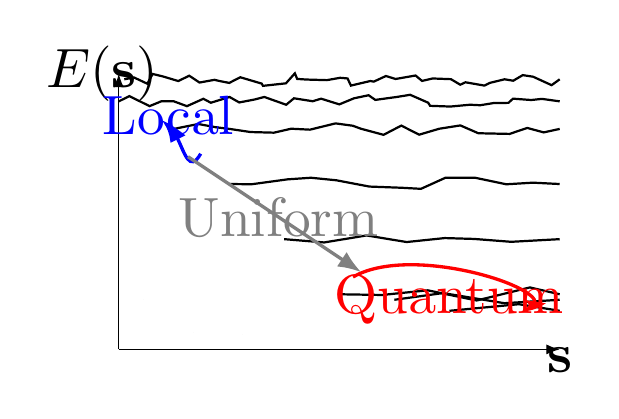
\begin{tikzpicture}[scale=0.7]
    \draw[arr](0,0)--(8,0);
    \node[scale=2] at (8,-.2){$\mathbf{s}$};
    \draw[arr](0,0)--(0,5);
    \node[scale=2] at (-.3,5){$E(\mathbf{s})$};
    \draw[decorate,decoration={random steps,segment length=4pt},thick] (0.1,4.9)--(7,4.9)--(8,4.9);
    \draw[decorate,decoration={random steps,segment length=5pt},thick](0,4.5)--(1,4.5)--(8,4.5);
    \draw[decorate,decoration={random steps,segment length=7pt},thick](1,4)--(8,4);
    \draw[decorate,decoration={random steps,segment length=10pt},thick](2,3)--(8,3);
    \draw[decorate,decoration={random steps,segment length=14pt},thick](3,2)--(8,2);
    \draw[decorate,decoration={random steps,segment length=17pt},thick](4,1)--(8,1);
    \draw[decorate,decoration={random steps,segment length=20pt},thick](5,.9)--(8,.9);
    \draw[decorate,decoration={random steps,segment length=24pt},thick](6,.7)--(8,.7);

    \filldraw[black,scale=.3] (1.5,3) circle;
    \filldraw[black,scale=.3] (4.5,1) circle;
    \filldraw[black,scale=.3] (7.5,.9) circle;
    
    \draw[bigarr,blue,very thick](1.4,3.4)to[out=-120,in=10] (.75,4.1); 
    \node[scale=2,blue] at (.9,4.25){Local}; 
    
    \draw[bigarr,red,very thick](4.4,1.4)to[out=30,in=10] (7.3,.7); 
    \node[scale=2,red] at (6,.9){Quantum}; 
    
    \draw[bigarr,gray,very thick](1.4,3.4)--(4.4,1.4); 
    \node[scale=2,gray] at (2.9,2.4){Uniform}; 
\end{tikzpicture}
\end{document}